\documentclass[/home/jesse/Analysis/FemtoAnalysis/AnalysisNotes/AnalysisNoteJBuxton.tex]{subfiles}
\begin{document}

\subsection{Spherical Harmonics}
\label{AdditionalFigures_SphericalHarmonics}



\begin{figure}[h]
  \centering
  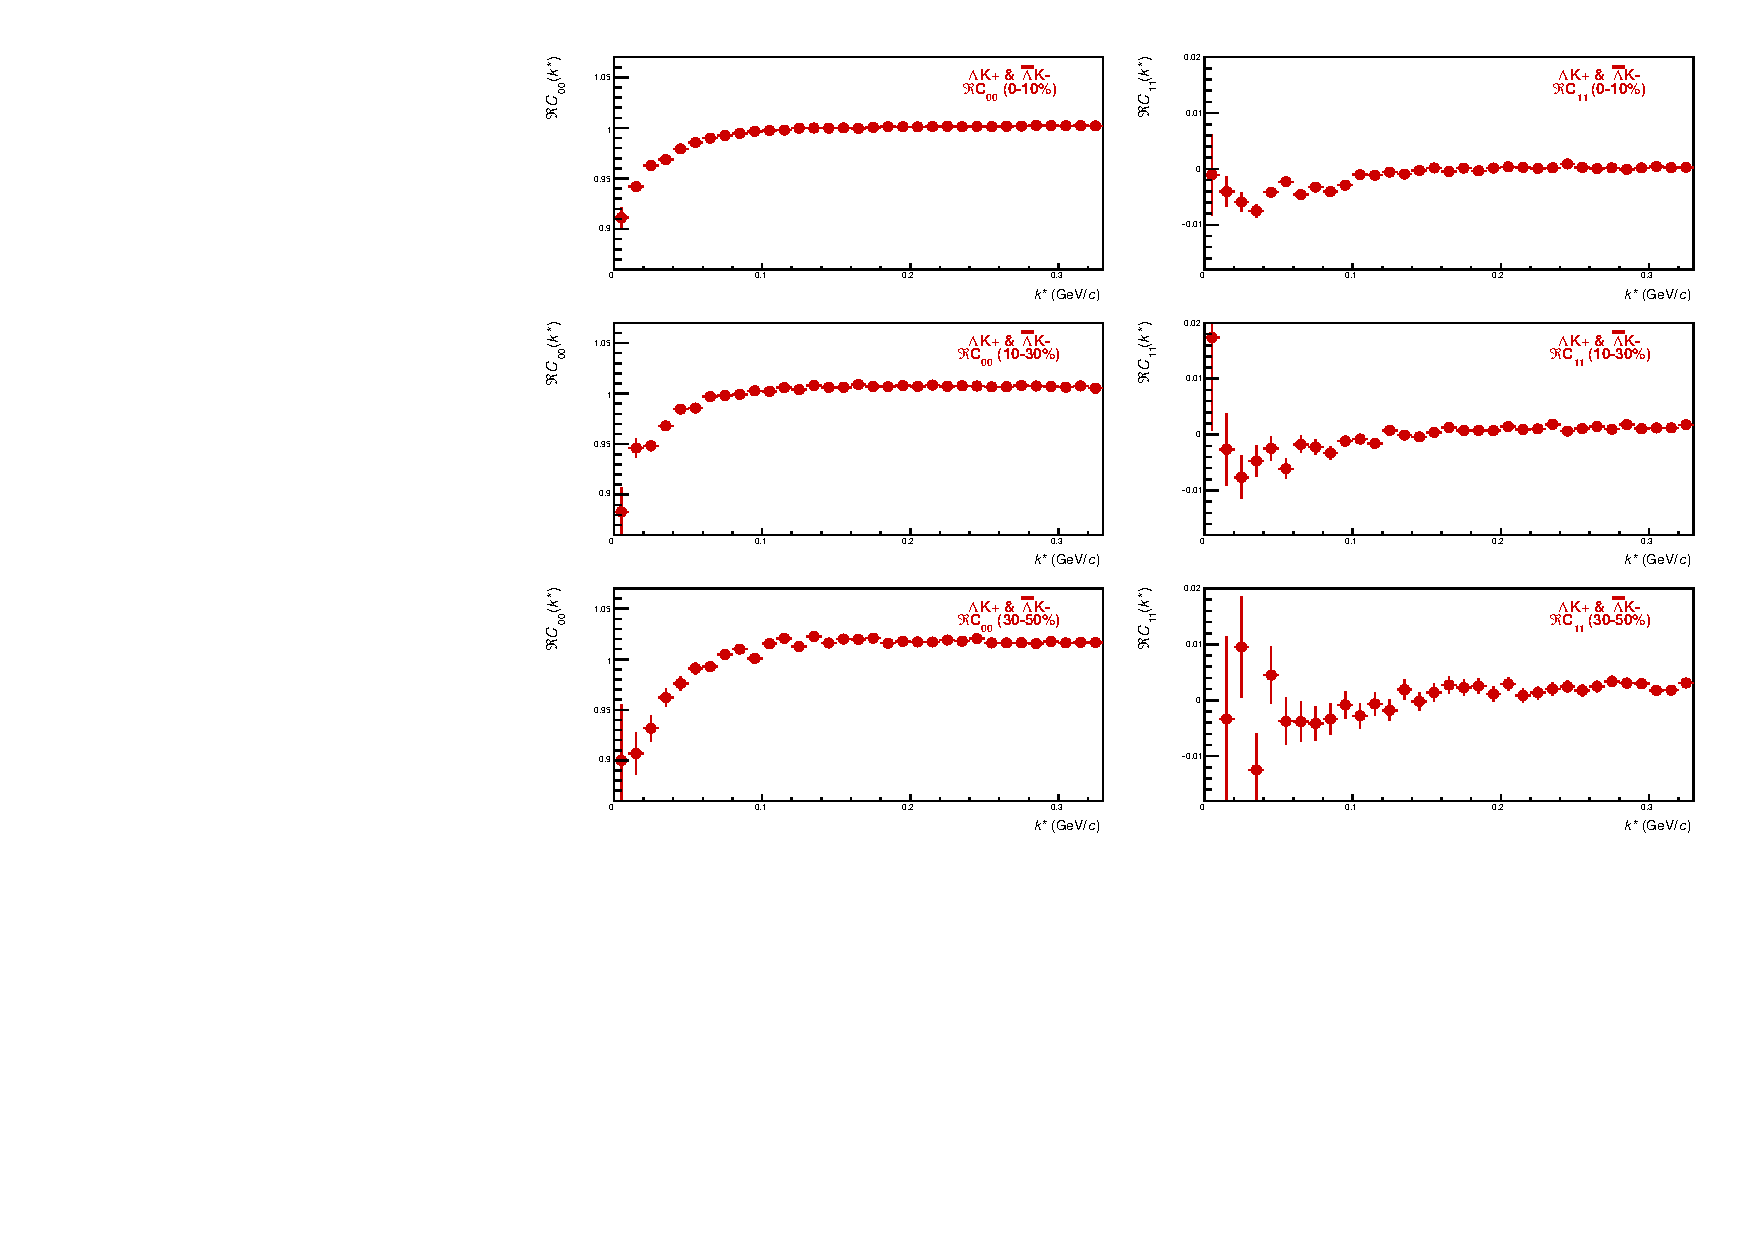
\includegraphics[width=\textwidth]{\ResultsDirBase Results_cLamcKch_20181205/SphericalHarmonics/LamKchP/CanCfYlmReC00C11_LamKchPALamKchM_All.pdf}
  \caption[\LamKchP $C_{00}$ and $\Im C_{11}$ Spherical Harmonic Components]{$C_{00}$ (left) and $\Im C_{11}$ (right) components of a spherical harmonic decomposition of the \LamKchP correlation function for the 0-10\% (top), 10-30\% (middle), and 30-50\% (bottom) centrality bins}
  \label{fig:LamKchP_ReC00C11_All}
\end{figure}



\begin{figure}[h!]
  \centering
  %%----start of first subfigure---  
  \subfloat[Real components, $\Re C_{lm}$]{
    \label{fig:LamKchP_FirstSixCYlm:a}
    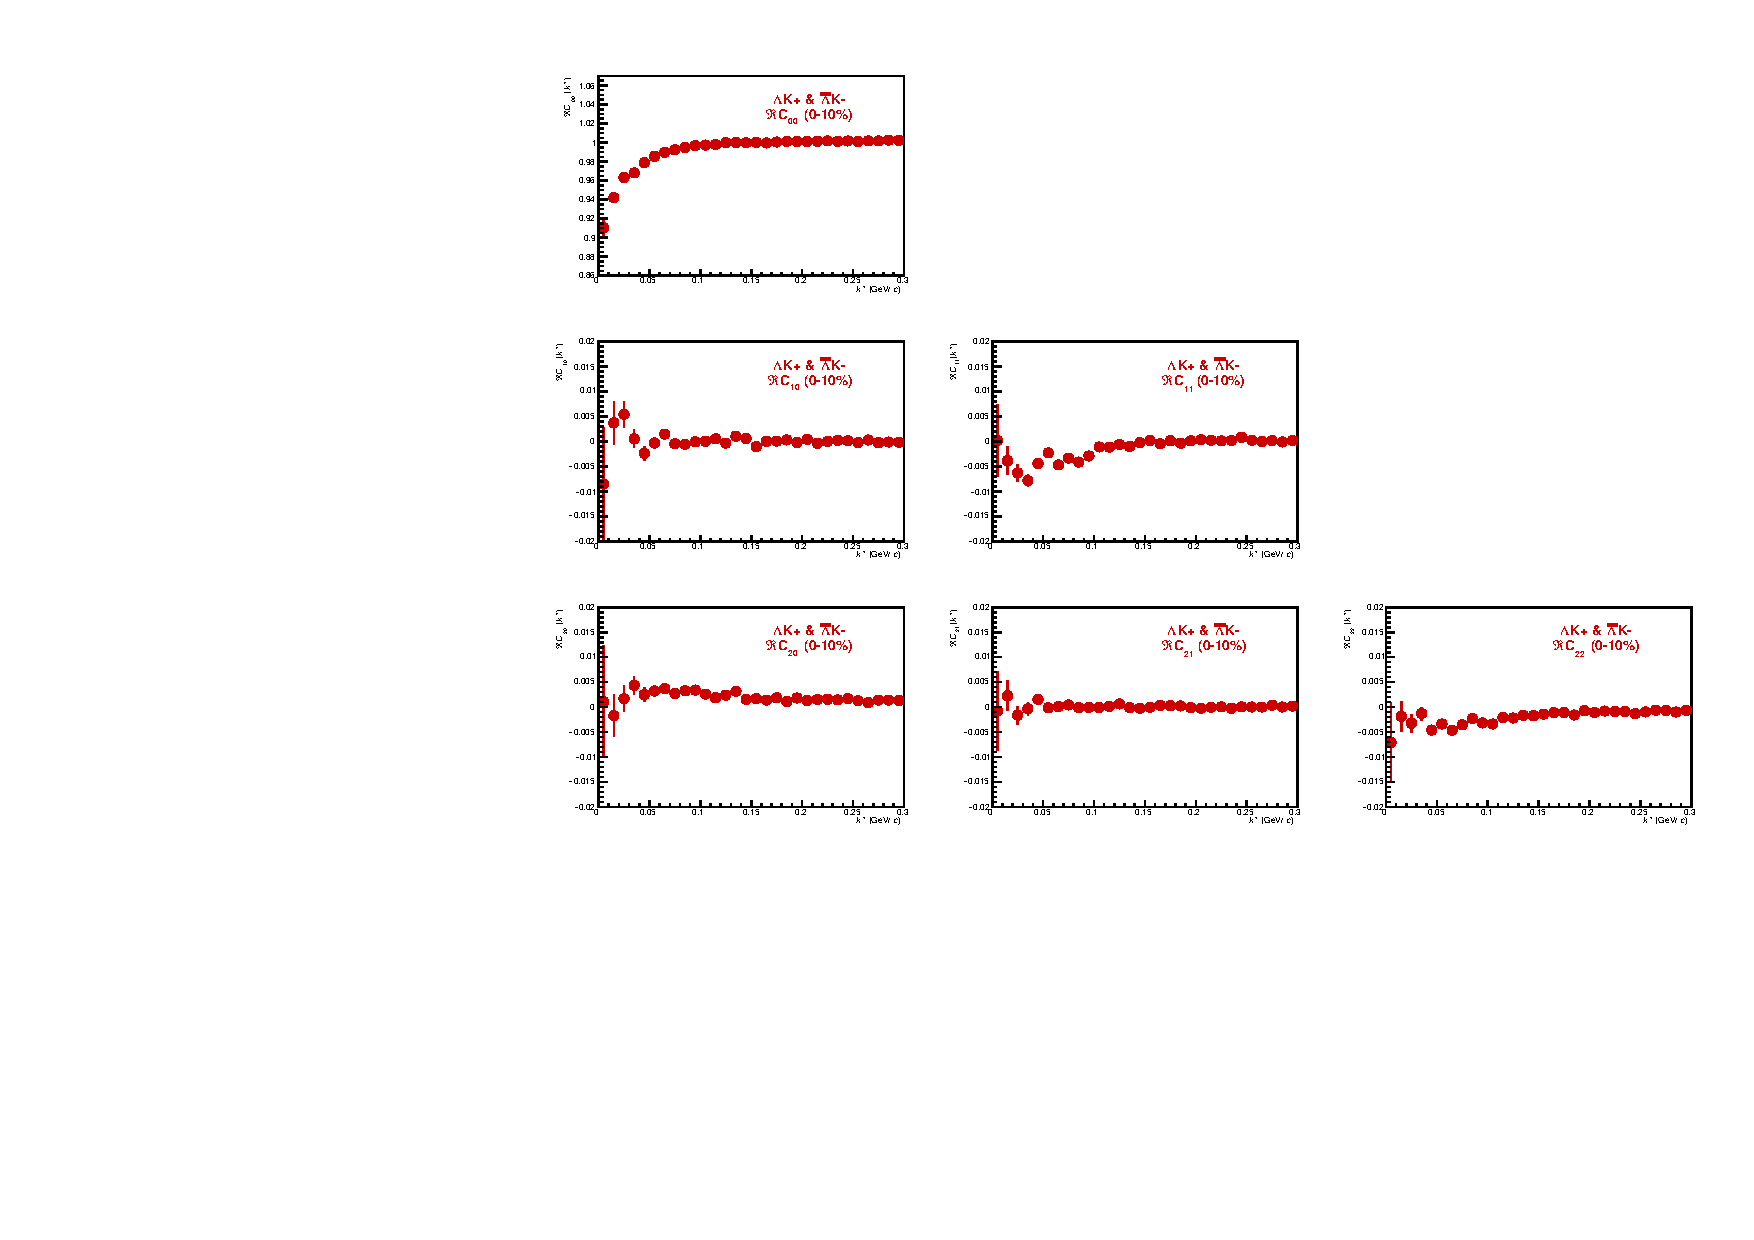
\includegraphics[width=\linewidth]{\ResultsDirBase Results_cLamcKch_20181205/SphericalHarmonics/LamKchP/CanCfYlmReFirstSixComps_LamKchPALamKchM_0010.pdf}} \\
  %%----start of second subfigure---
  \subfloat[Imaginary components, $\Im C_{lm}$]{
    \label{fig:LamKchP_FirstSixCYlm:b}
    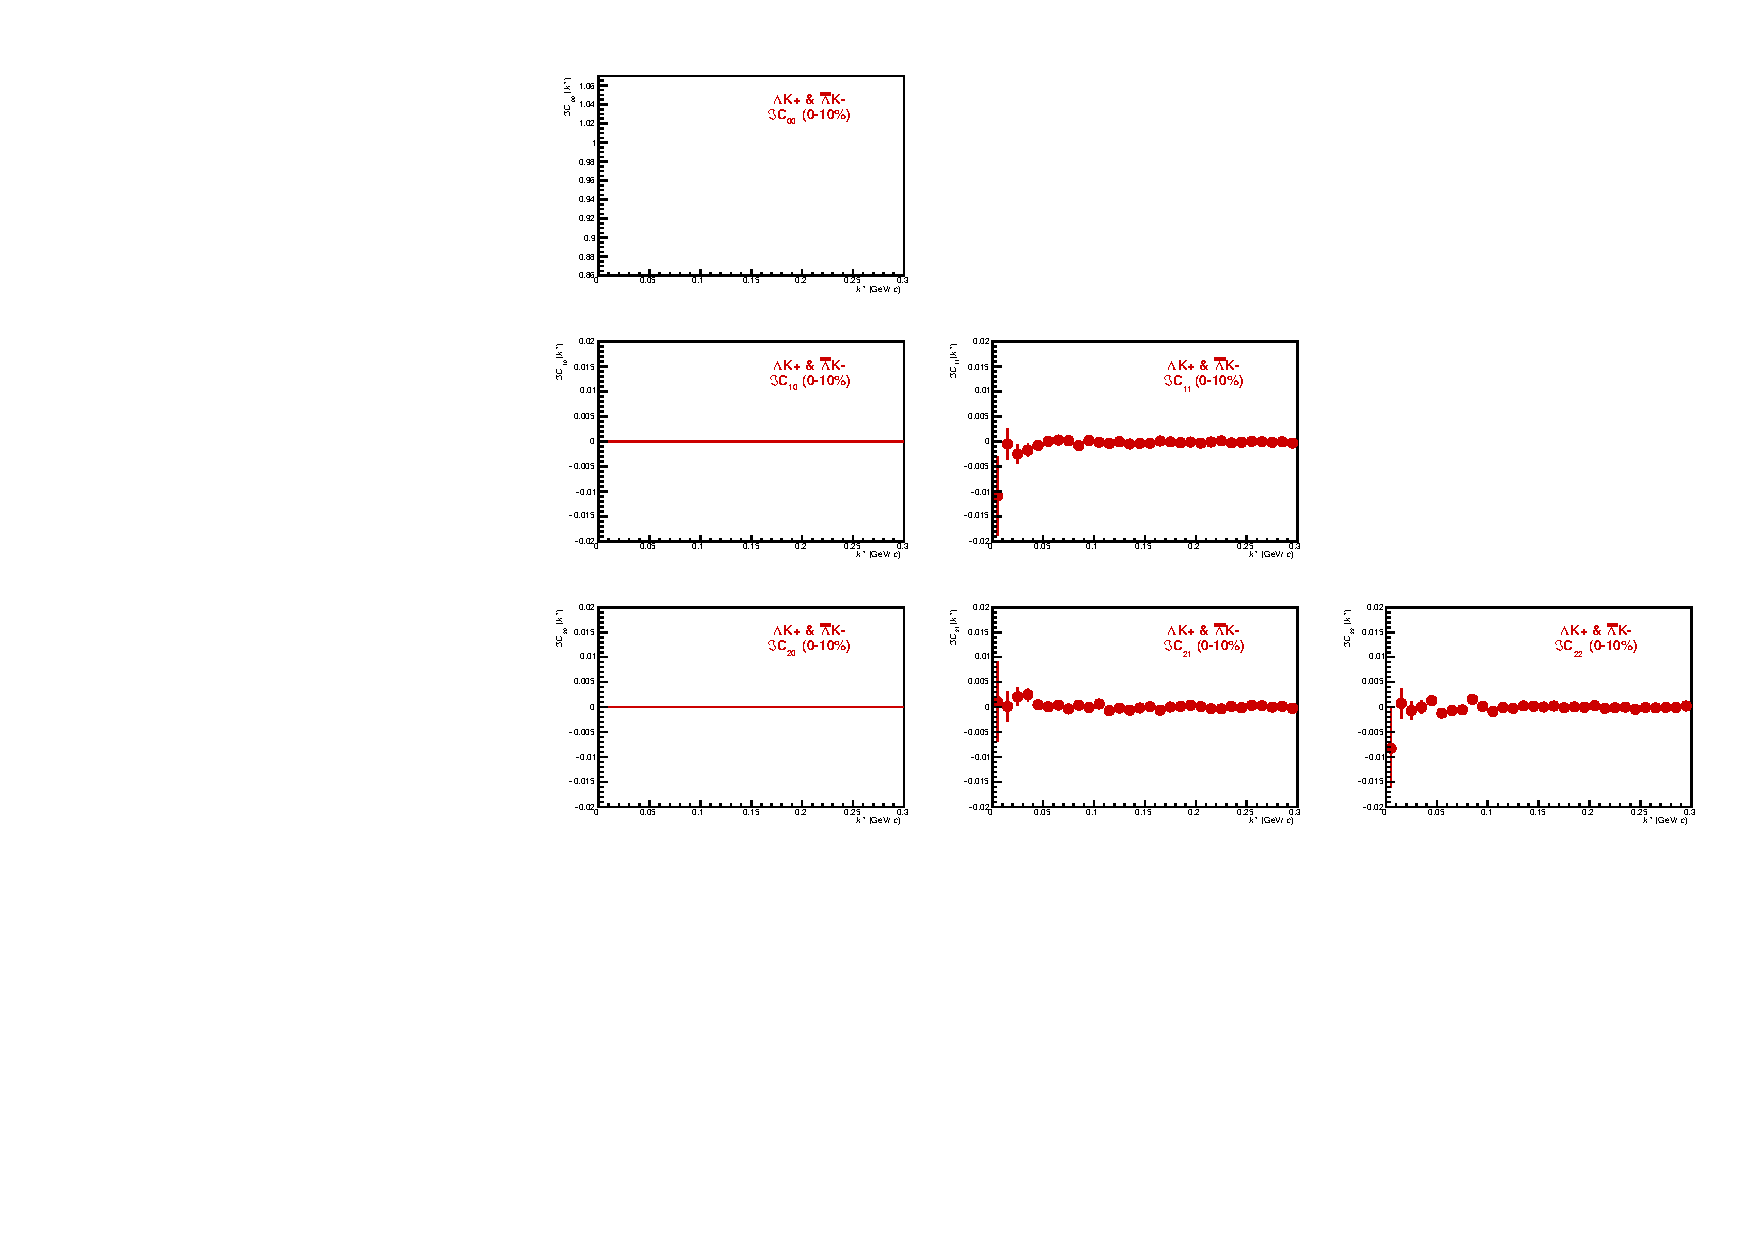
\includegraphics[width=\linewidth]{\ResultsDirBase Results_cLamcKch_20181205/SphericalHarmonics/LamKchP/CanCfYlmImFirstSixComps_LamKchPALamKchM_0010.pdf}}  
  %%----overall caption----
  \caption[\LamKchP First Six Components of Spherical Harmonic Decomposition (0-10\%)]{First six components ($C_{00}, C_{10}, C_{11}, C_{20}, C_{21}, C_{22}$) of the spherical harmonic decomposition of the \LamKchP correlation function for the 0-10\% centrality bin.
  Note, $\Im C_{00}$, $\Im C_{10}$, and $\Im C_{20}$ are zero by definition.}
  \label{fig:LamKchP_FirstSixCYlm}
\end{figure}











\begin{figure}[h]
  \centering
  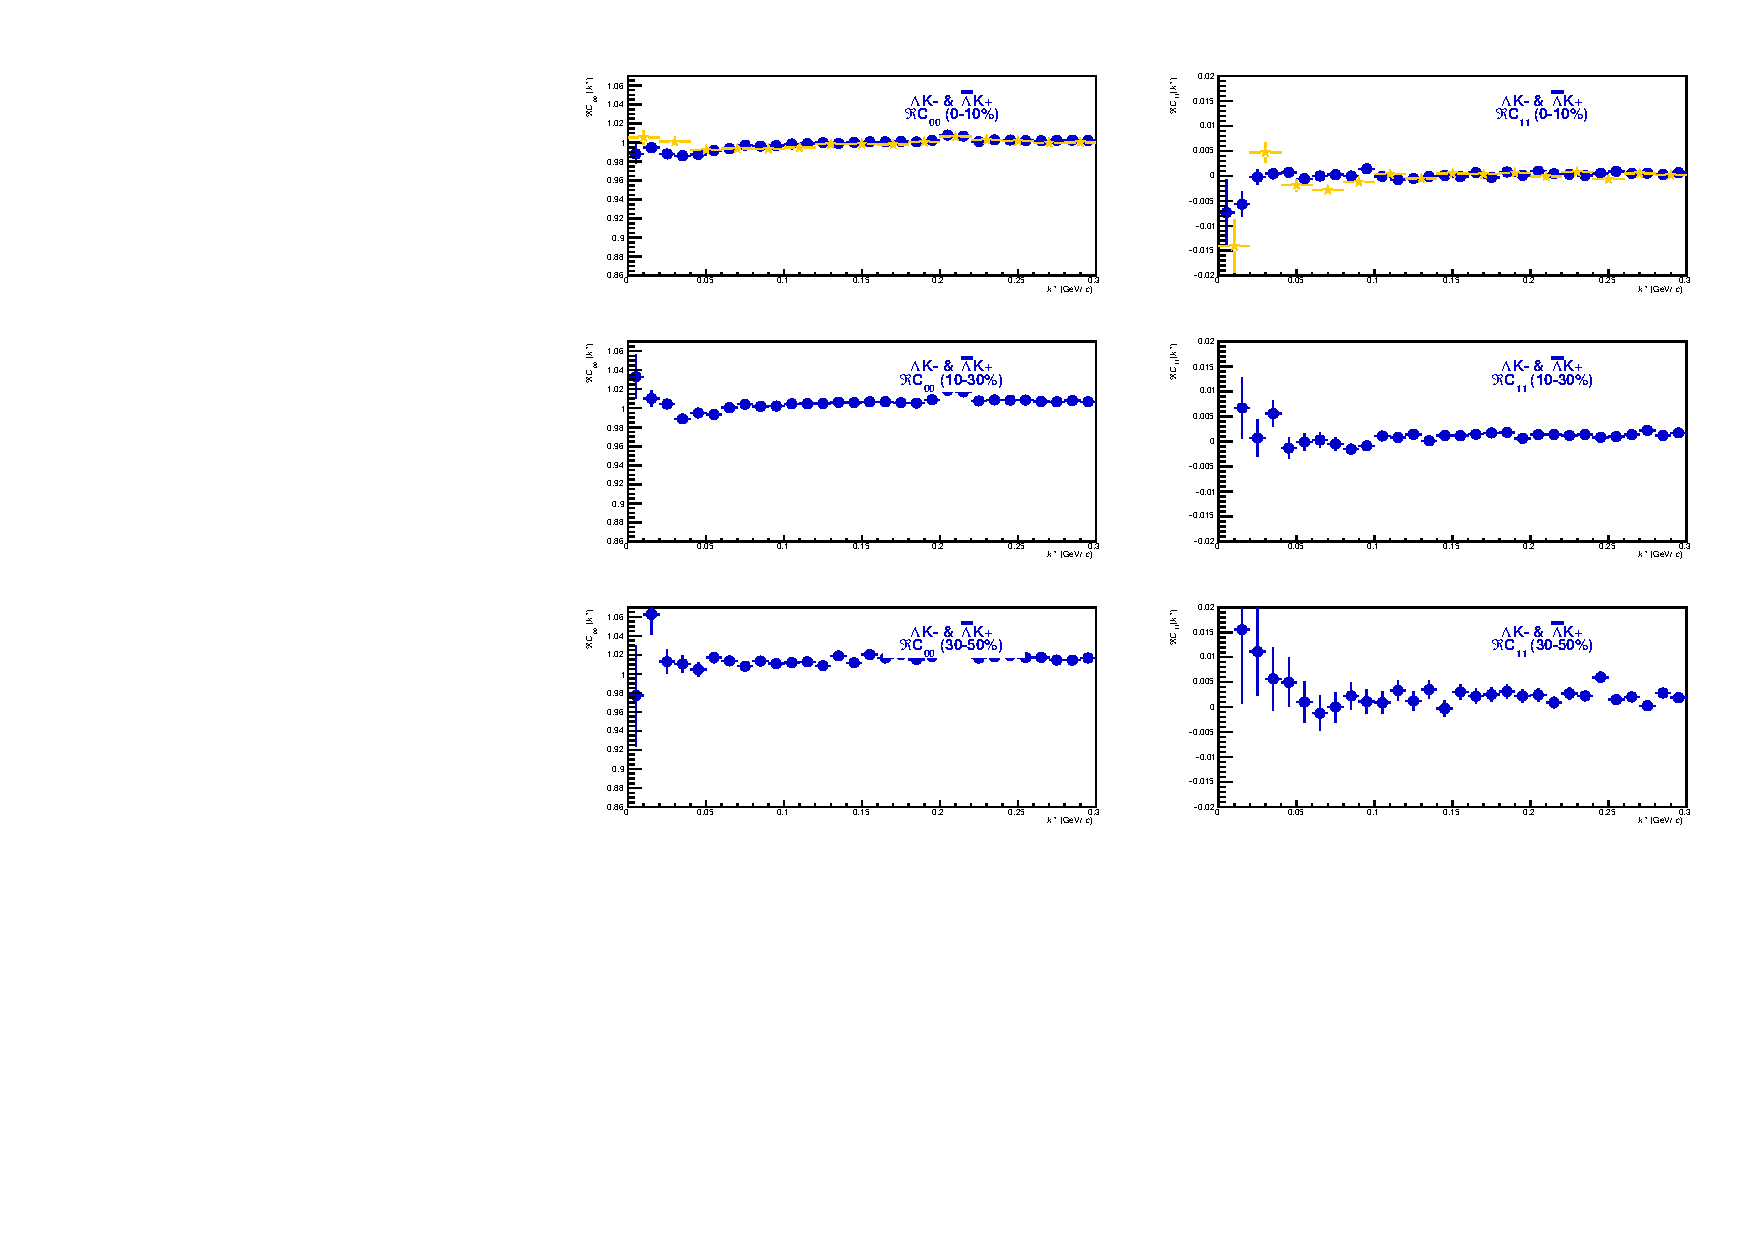
\includegraphics[width=\textwidth]{\ResultsDirBase Results_cLamcKch_20181205/SphericalHarmonics/LamKchM/CanCfYlmReC00C11_LamKchMALamKchP_All.pdf}
  \caption[\LamKchM $C_{00}$ and $\Im C_{11}$ Spherical Harmonic Components]{$C_{00}$ (left) and $\Im C_{11}$ (right) components of a spherical harmonic decomposition of the \LamKchM correlation function for the 0-10\% (top), 10-30\% (middle), and 30-50\% (bottom) centrality bins}
  \label{fig:LamKchM_ReC00C11_All}
\end{figure}



\begin{figure}[h!]
  \centering
  %%----start of first subfigure---  
  \subfloat[Real components, $\Re C_{lm}$]{
    \label{fig:LamKchM_FirstSixCYlm:a}
    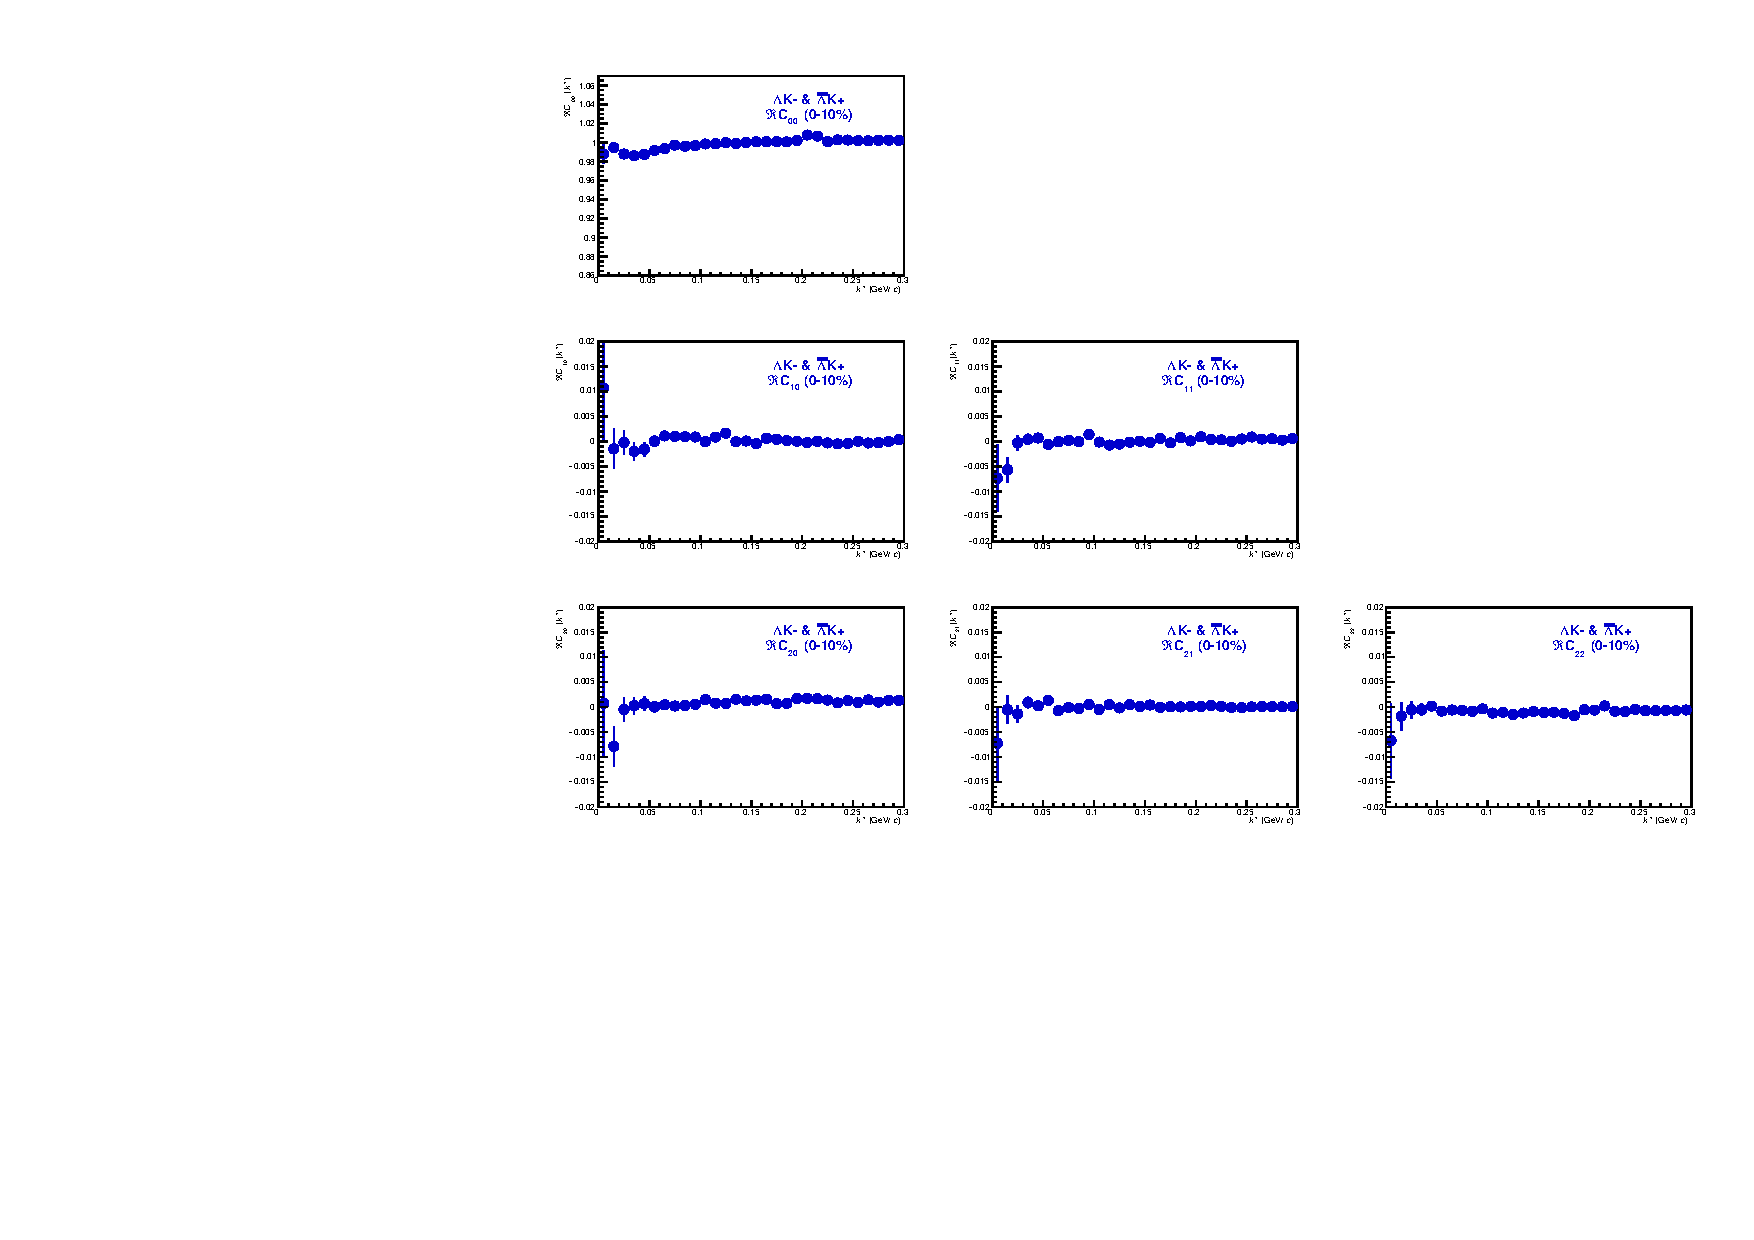
\includegraphics[width=\linewidth]{\ResultsDirBase Results_cLamcKch_20181205/SphericalHarmonics/LamKchM/CanCfYlmReFirstSixComps_LamKchMALamKchP_0010.pdf}} \\
  %%----start of second subfigure---
  \subfloat[Imaginary components, $\Im C_{lm}$]{
    \label{fig:LamKchM_FirstSixCYlm:b}
    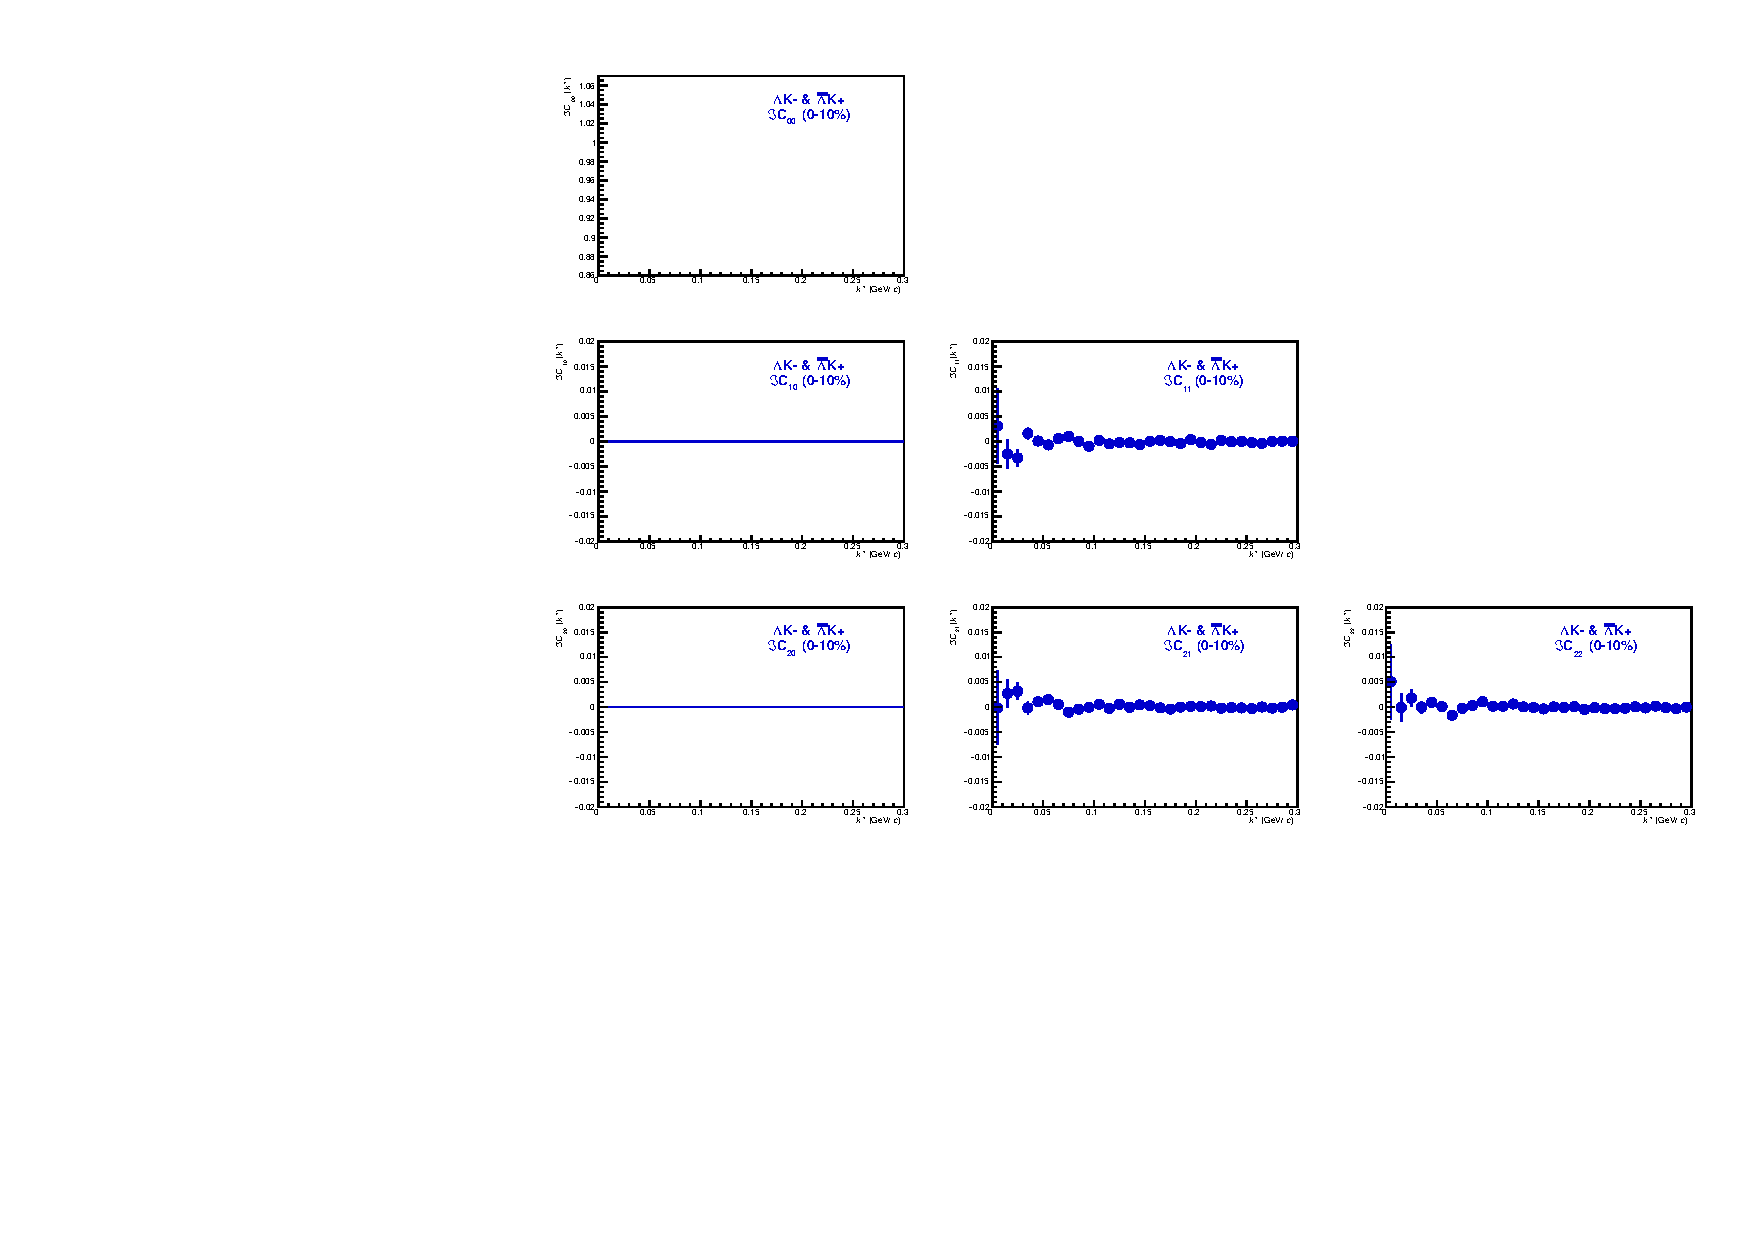
\includegraphics[width=\linewidth]{\ResultsDirBase Results_cLamcKch_20181205/SphericalHarmonics/LamKchM/CanCfYlmImFirstSixComps_LamKchMALamKchP_0010.pdf}}  
  %%----overall caption----
  \caption[\LamKchM First Six Components of Spherical Harmonic Decomposition (0-10\%)]{First six components ($C_{00}, C_{10}, C_{11}, C_{20}, C_{21}, C_{22}$) of the spherical harmonic decomposition of the \LamKchM correlation function for the 0-10\% centrality bin.
  Note, $\Im C_{00}$, $\Im C_{10}$, and $\Im C_{20}$ are zero by definition.}
  \label{fig:LamKchM_FirstSixCYlm}
\end{figure}













\begin{figure}[h]
  \centering
  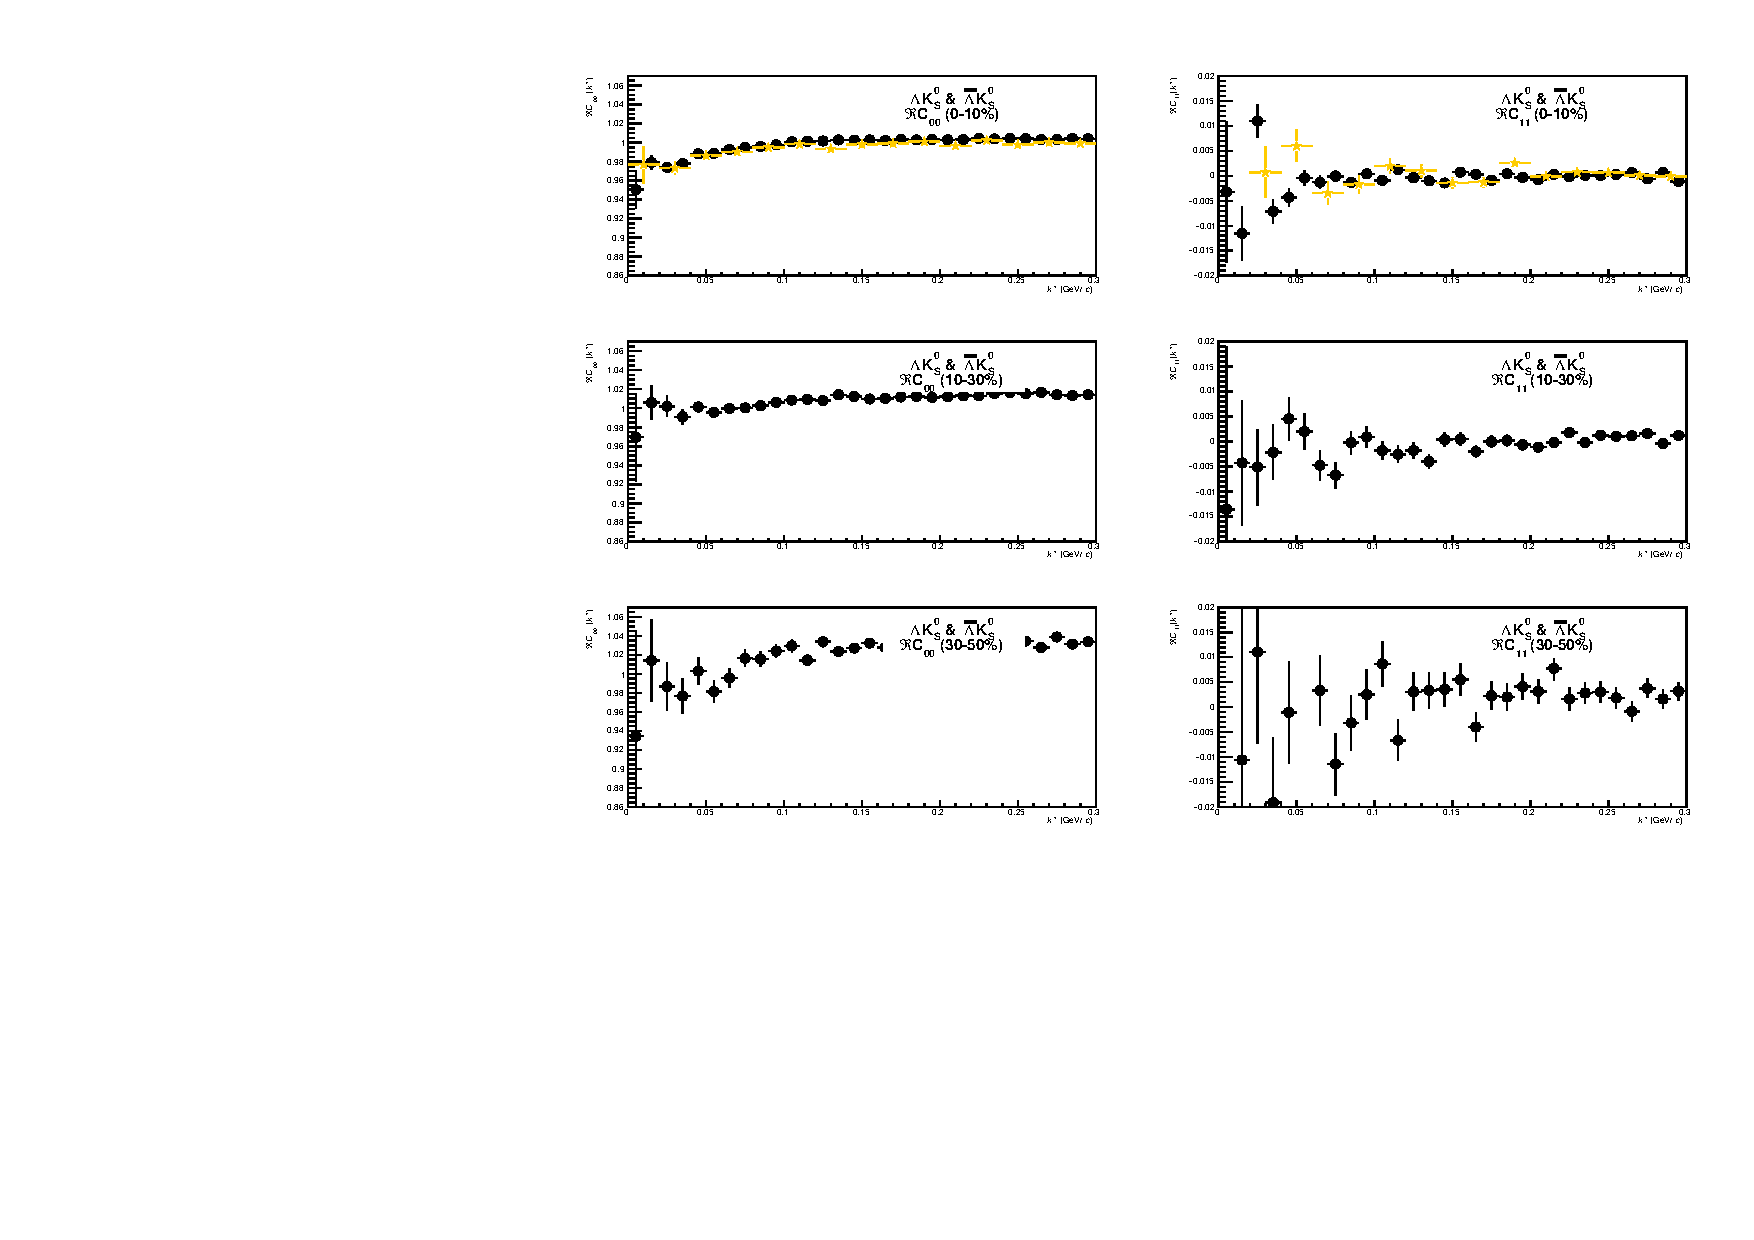
\includegraphics[width=\textwidth]{\ResultsDirBase Results_cLamK0_20181205/SphericalHarmonics/LamK0/CanCfYlmReC00C11_LamK0ALamK0_All.pdf}
  \caption[\LamKs $C_{00}$ and $\Im C_{11}$ Spherical Harmonic Components]{$C_{00}$ (left) and $\Im C_{11}$ (right) components of a spherical harmonic decomposition of the \LamKs correlation function for the 0-10\% (top), 10-30\% (middle), and 30-50\% (bottom) centrality bins}
  \label{fig:LamK0_ReC00C11_All}
\end{figure}



\begin{figure}[h!]
  \centering
  %%----start of first subfigure---  
  \subfloat[Real components, $\Re C_{lm}$]{
    \label{fig:LamK0_FirstSixCYlm:a}
    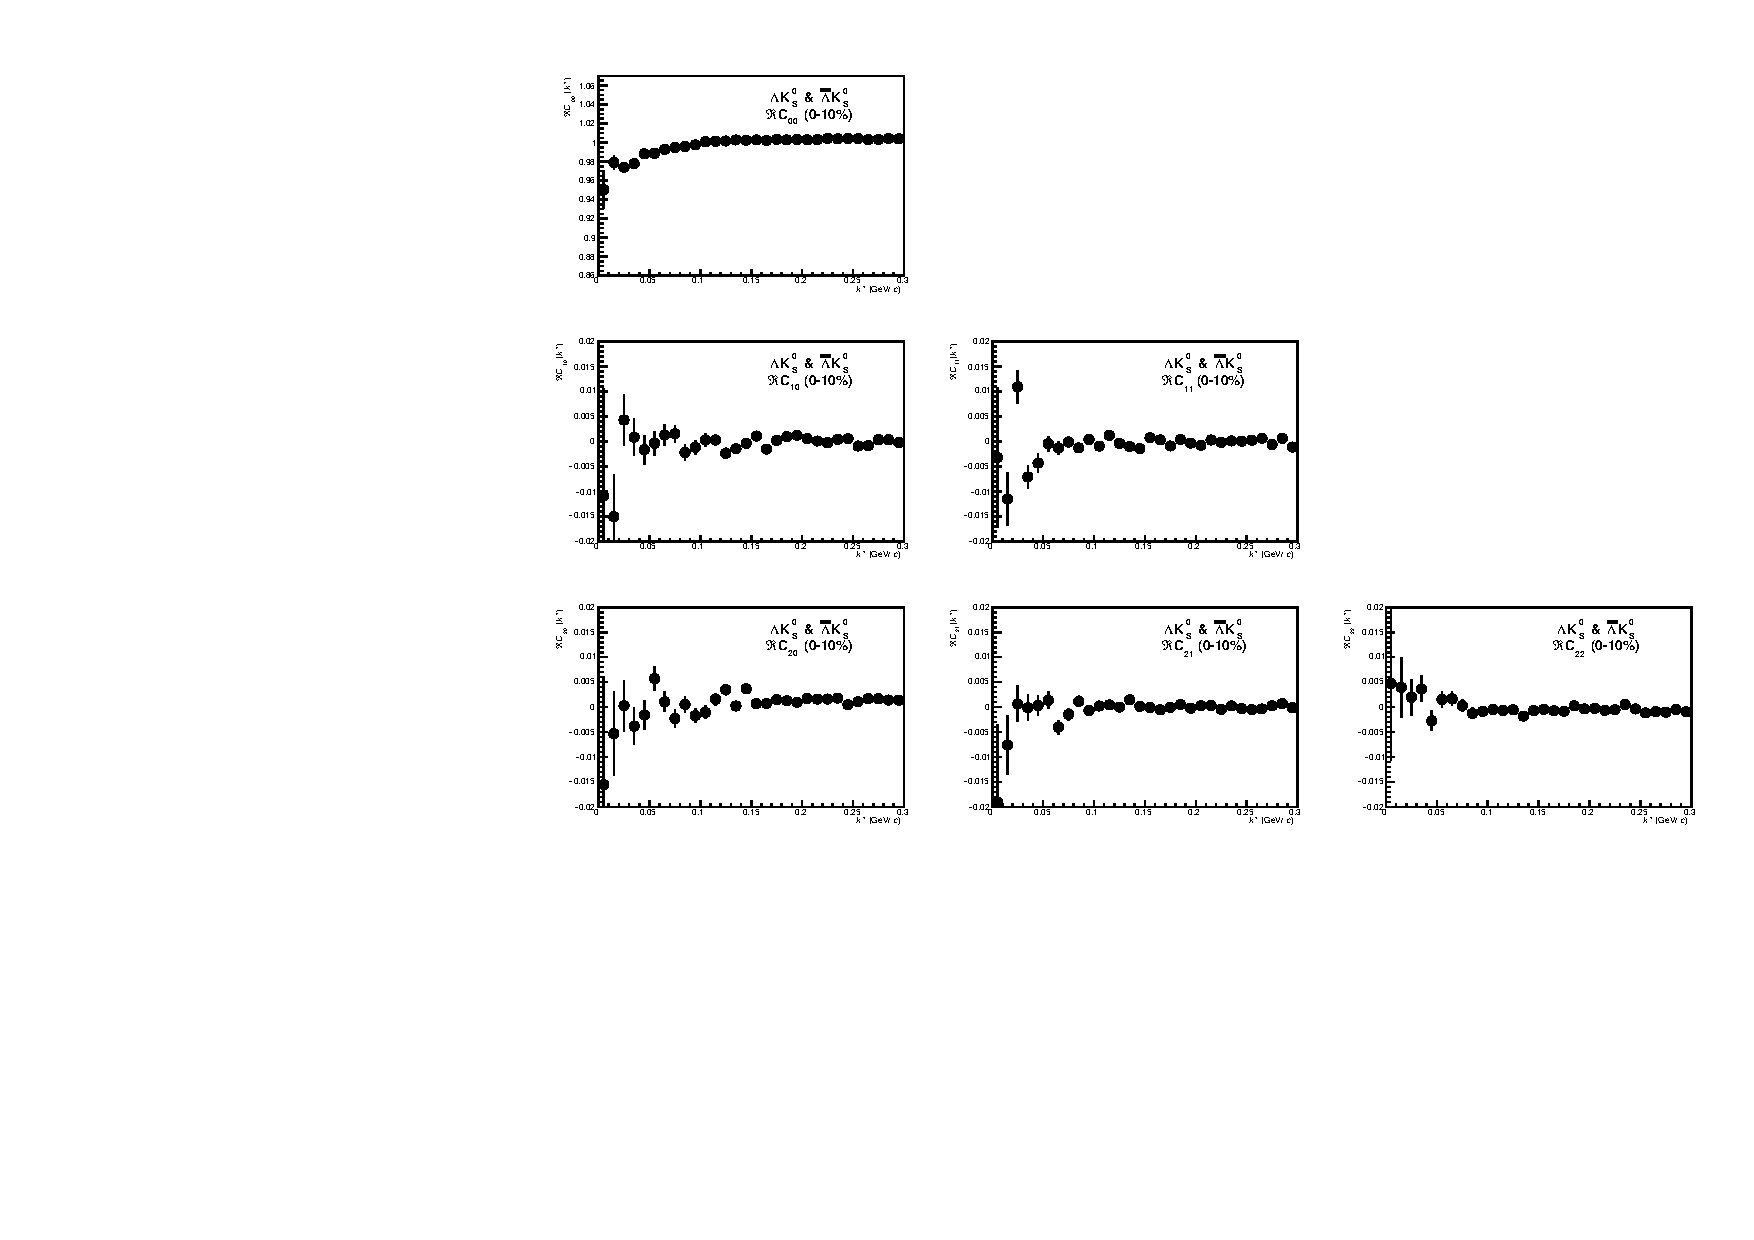
\includegraphics[width=\linewidth]{\ResultsDirBase Results_cLamK0_20181205/SphericalHarmonics/LamK0/CanCfYlmReFirstSixComps_LamK0ALamK0_0010.pdf}} \\
  %%----start of second subfigure---
  \subfloat[Imaginary components, $\Im C_{lm}$]{
    \label{fig:LamK0_FirstSixCYlm:b}
    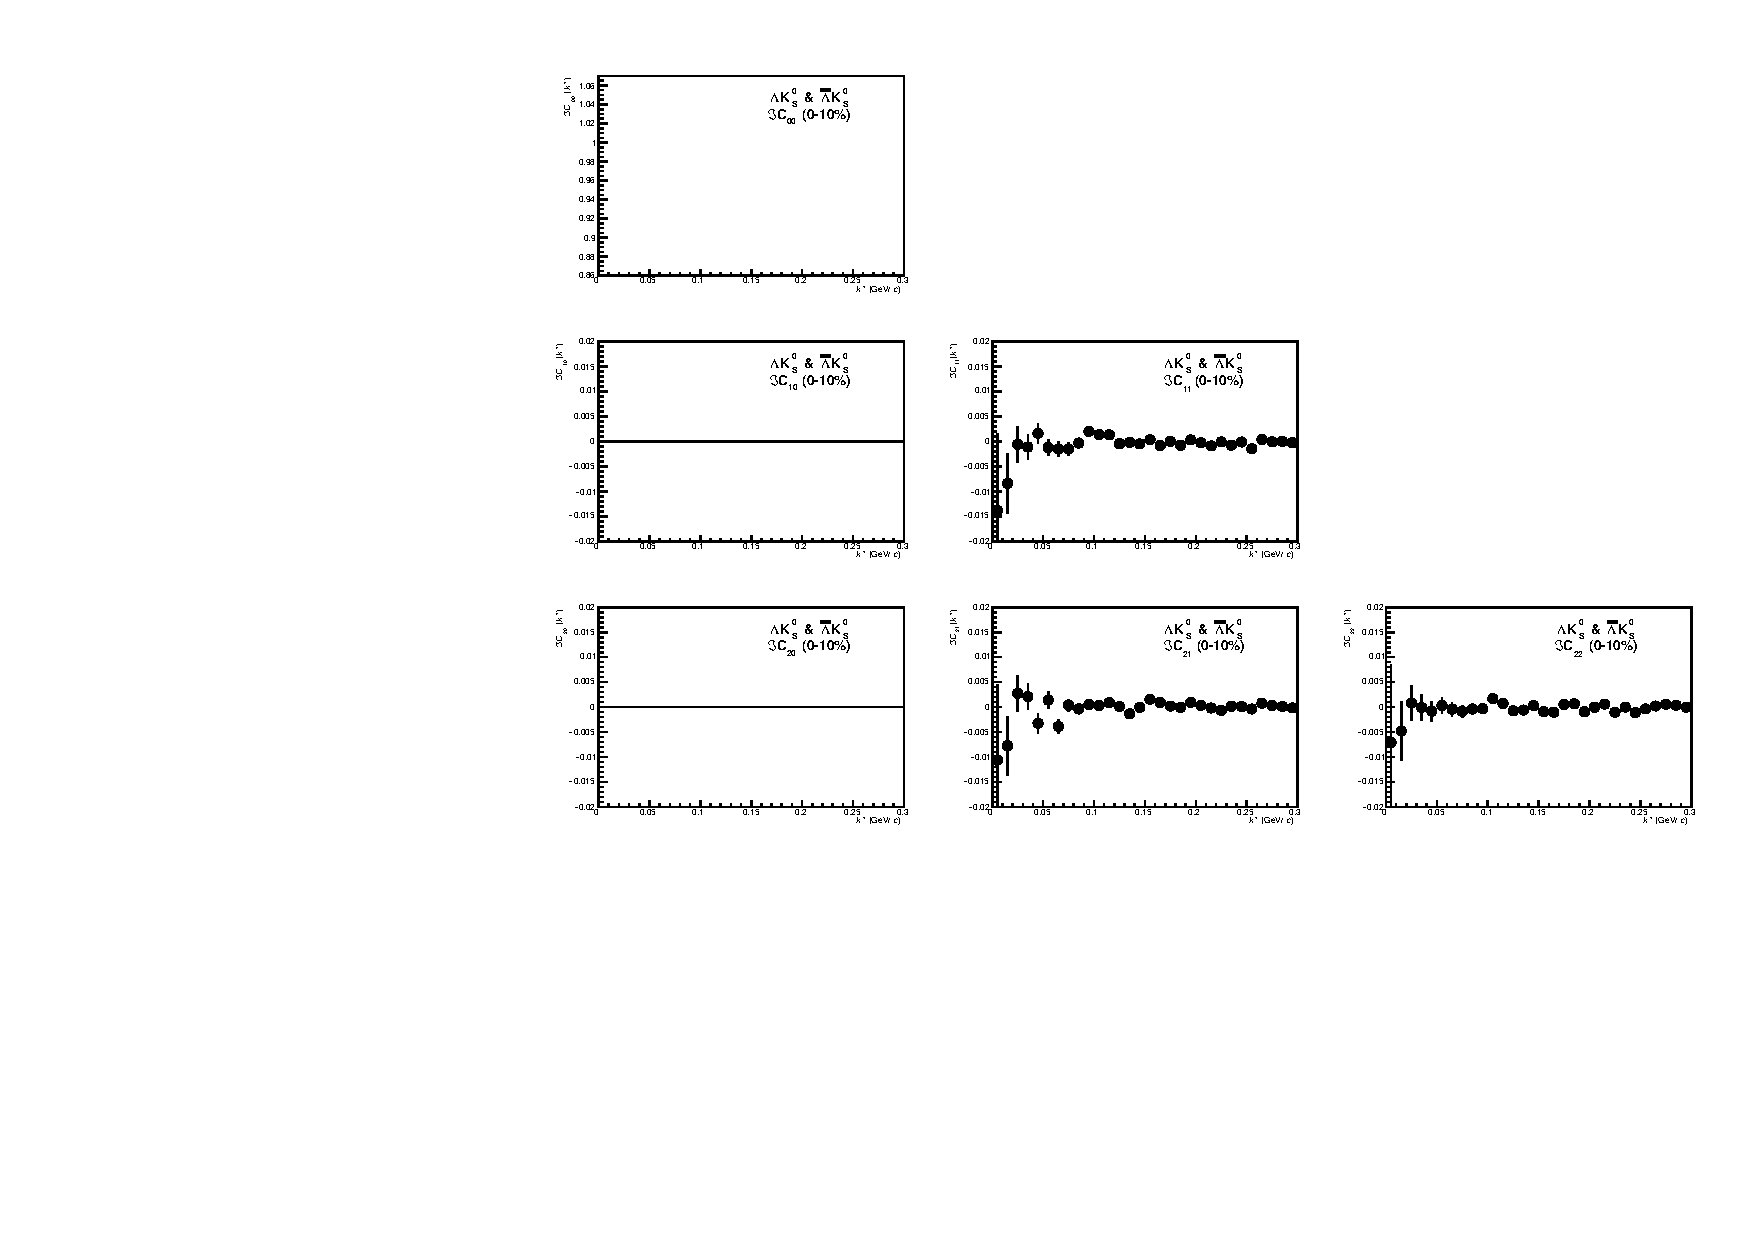
\includegraphics[width=\linewidth]{\ResultsDirBase Results_cLamK0_20181205/SphericalHarmonics/LamK0/CanCfYlmImFirstSixComps_LamK0ALamK0_0010.pdf}}  
  %%----overall caption----
  \caption[\LamKs First Six Components of Spherical Harmonic Decomposition (0-10\%)]{First six components ($C_{00}, C_{10}, C_{11}, C_{20}, C_{21}, C_{22}$) of the spherical harmonic decomposition of the \LamKs correlation function for the 0-10\% centrality bin.
  Note, $\Im C_{00}$, $\Im C_{10}$, and $\Im C_{20}$ are zero by definition.}
  \label{fig:LamK0_FirstSixCYlm}
\end{figure}

\end{document}